\documentclass[10pt,a4paper]{report}
\usepackage[latin1]{inputenc}
\usepackage{amsmath}
\usepackage{amsfonts}
\usepackage{amssymb}
\usepackage{graphicx}
\usepackage[left=2.00cm, right=2.00cm, top=2.00cm, bottom=2.00cm]{geometry}
\usepackage[spanish]{babel}  %Cambia las etiquetas a espa�ol 
\usepackage{multicol}
\usepackage{wrapfig}
\usepackage{subfig}	%Varias imagenes
\usepackage[hidelinks]{hyperref} %URL
% Bibliography
\newcommand{\HRule}{\rule{\linewidth}{0.5mm}}
\usepackage[style=alphabetic,sorting=nyt,sortcites=true,autopunct=true,babel=hyphen,hyperref=true,abbreviate=false,backref=true,backend=biber]{biblatex}
\addbibresource{referenciasBibliograficas.bib} % BibTeX bibliography file
\defbibheading{bibempty}{}
\usepackage[table]{xcolor} %Filas 
\definecolor{grisClaro}{RGB}{229,229,229}


\begin{document}
	
\begin{titlepage}
\begin{center}

% Upper part of the page. The '~' is needed because \\
% only works if a paragraph has started.

\includegraphics[width=0.25\textwidth]{./source/logoescom}~\\[1.5cm]

\textsc{\LARGE ESCUELA SUPERIOR DE C�MPUTO}\\[1.5cm]

\textsc{\Large Trabajo Terminal I\\ \textbf{2014-A039}}\\[0.5cm]

% Title
\HRule \\[0.4cm]
{ \huge \bfseries Sistema de Gesti�n y Localizaci�n de Estacionamientos Cercanos Para Usuarios M�viles \\[0.4cm] }
\HRule \\[3cm]

% Author and supervisor

{\Large \textbf{Alumnos}}\\[.5cm]
{\Large \textit{Jesus Manuel Ram�rez Obeso}}\\
{\Large \textit{Jos� Miguel Res�ndiz Garc�a} }\\[1cm]


{\Large \textbf{Directores}}\\[.5cm]
{\Large \textit{Dr. Santiago Miguel Su�rez Casta��n} }\\
{\Large \textit{M. en C. Jos� Asunci�n Enriquez Z�rate}}\\[1cm]



\vfill

% Bottom of the page
{\large \today}

\end{center}
\end{titlepage}
	\tableofcontents
	\chapter{Estudio de Mercado}
		\section{Definici�n Del Problema}
			En la actualidad se ha vuelto un problema cotidiano encontrar un lugar disponible en un estacionamiento, principalmente en zonas comerciales, de oficinas o de gran actividad econ�mica. Es com�n que un conductor (usuario) vaya a un estacionamiento en espec�fico y no encuentre un espacio disponible, lo cual puede hacer que pierda un tiempo considerable en encontrar un lugar disponible. 

Una investigaci�n realizada por el Instituto de Pol�ticas para el Transporte y el Desarrollo (ITDP), revel� que en �reas d�nde la oferta de estacionamientos no es suficiente para cubrir la demanda y se ofrecen espacios de estacionamiento en v�a p�blica de manera gratuita, se generan efectos negativos que afectan a residentes y visitantes \cite{ITDP}.

\begin{figure}[h]
	\centering
	\includegraphics[scale=.25]{./definicionDelProblema/source/trafico.pdf}
	\caption{Problemas cotidianos por falta disponibilidad en estacionamietos}
	\label{fig:ProblemasCotidianos}
\end{figure}

\begin{itemize}
	\item Baja disponibilidad de estacionamientos
	\item Estacionamientos ilegales
	\item Apropiaci�n ilegal de estacionamientos
	\item Altos niveles de ruido y contaminaci�n
	\item Congesti�n vial y tiempos de b�squeda largos en estacionamientos	
\end{itemize}


Por otro lado en estacionamientos(administradores) peque�os y medianos los ingresos no son suficientes para la adquisici�n de un sistema o la contrataci�n de  un  agente  externo  que  realice  dichas  administraci�n;  incluso  para  estacionamientos  grandes  con  mayores  ingresos  la implementaci�n de un sistema, automatizaci�n u outsourcing disminuye en gran medida sus ingresos.
		\section{Definici�n Del Producto}	
			Una plataforma en la Nube para la administraci�n y localizaci�n de estacionamiento (SAE) capaz de ajustarse a las necesidades de las diferentes modalidades de estacionamientos  p�blicos y privados del Distrito  Federal como son estacionamiento, parqu�metros, valet-parking y  pensiones.  Permitir�  gestionar  y  realizar  las  tareas operativas y administrativas que se realizan de manera general en un estacionamiento. Figura \ref{fig:ArquitecturaGeneralSAE}

\begin{figure}[h]
	\centering
	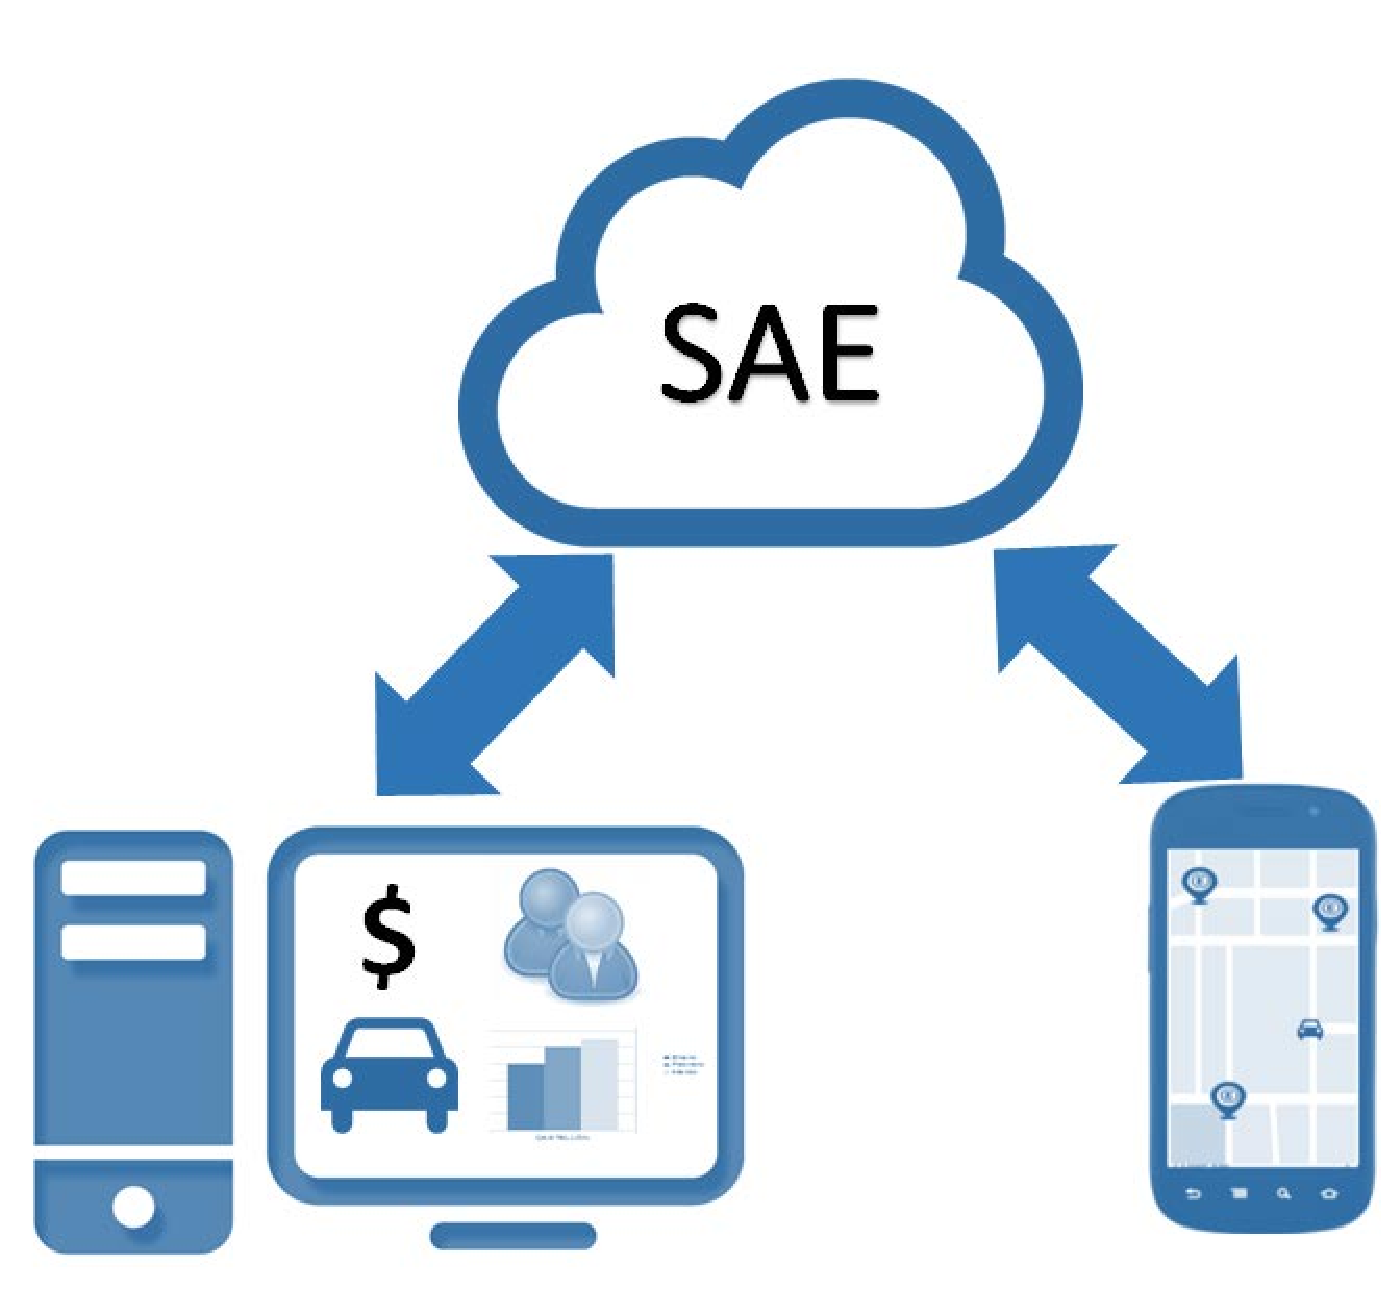
\includegraphics[scale=.4]{./definicionDelProducto/source/arquitecturaSAE.pdf}
	\caption{Arquitectura general SAE}
	\label{fig:ArquitecturaGeneralSAE}
\end{figure}		 

La informaci�n de los estacionamientos en operaci�n podr� ser visualizada por los usuarios finales a trav�s de una app m�vil de manera f�cil. Esta mostrar� en un mapa los estacionamientos cercamos, n�mero de cajones disponibles, horarios, modos de cobro, tarifas, y una calificaci�n.Figura \ref{fig:usuarioAppLocalizacion}

\begin{figure}[ht]
	\centering
	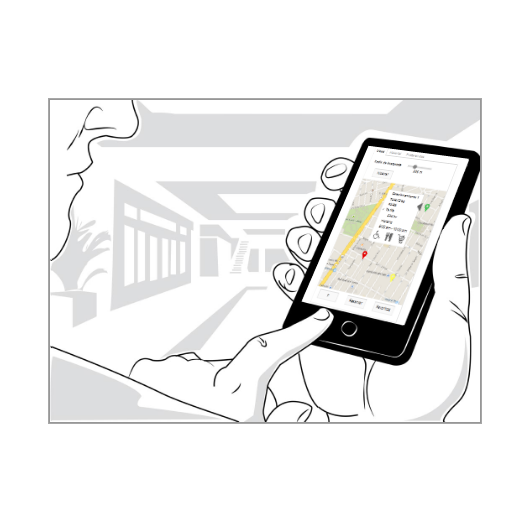
\includegraphics[scale=0.4]{./definicionDelProducto/source/usuarioApp}
	\caption{App de localizaci�n}
	\label{fig:usuarioAppLocalizacion}
\end{figure}

\newpage
La Figura \ref{fig:EscenarioSAE} ejemplifica el escenario principal de uso del SAE.

\begin{figure}[ht]
	\centering
	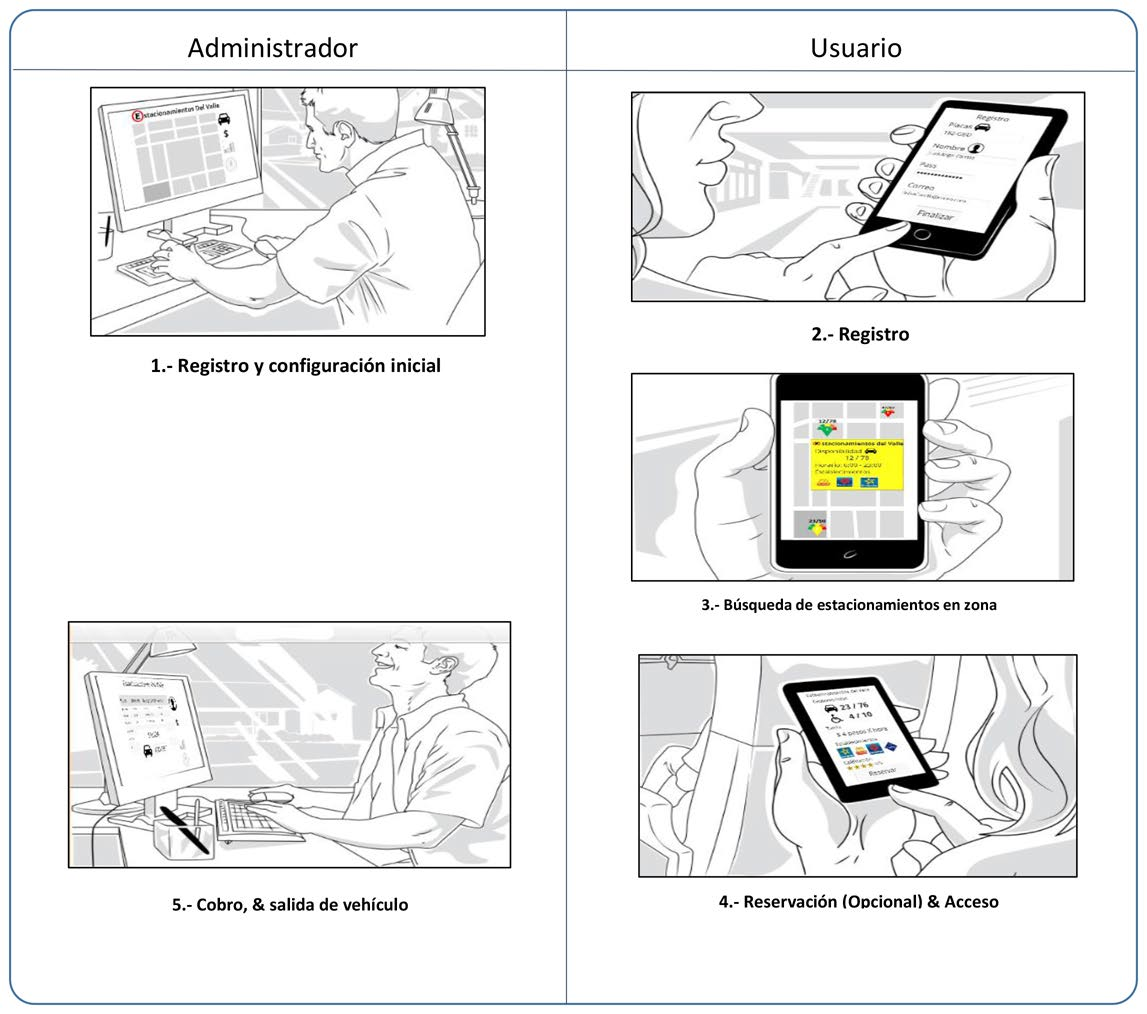
\includegraphics[scale=0.75]{./definicionDelProducto/source/storyboard.pdf}
	\caption{Escenario de uso SAE}
	\label{fig:EscenarioSAE}
\end{figure}

 Las principales caracteristicas del la plataforma son:
\begin{itemize}
	\item Configuraci�n f�sica
		\begin{itemize}
			\item N�mero de niveles
			\item N�mero de cajones
			\item Cajones para personas con capacidades diferectes.
			\item Ubicac�n del estacionamiento 
			\item Horario de operaci�n
			\item Modalidad(Pensi�n, valet, normal)
			\item Publico o Privado
		\end{itemize}
	\item Control de entradas y salidas
	\item Control de ususarios
	\item Generaci�n de reportes
	\item Consultas
	\item Configuraci�n de tarifas
	\item Agregar servicios adicionales (lavado, aspirado, pulido, Etc.)
	\item API de integraci�n para otros sistemas
	\item App de localizai�n de estacionamientos
\end{itemize}

	



		\section{An�lisis De La Demanda}
			\subsection{CONSUMIDORES DIRECTOS}

Se consideran consumidores directos a los administradores o due�os de estacionamiento. De acuerdo a una investigaci�n realizada por la UNAM. En el DF hay 1,783 estacionamientos p�blicos, con m�s de 300 mil cajones \cite{publimetro}. La Figura \ref{fig:graficaEstacionamientosPorArea} muestras las 6 delegaciones (m�s de 84\% del total) con mayor n�mero de estacionamiento, asi como, el porcentaje que le corresponde.

\begin{figure}[ht]
	\centering
	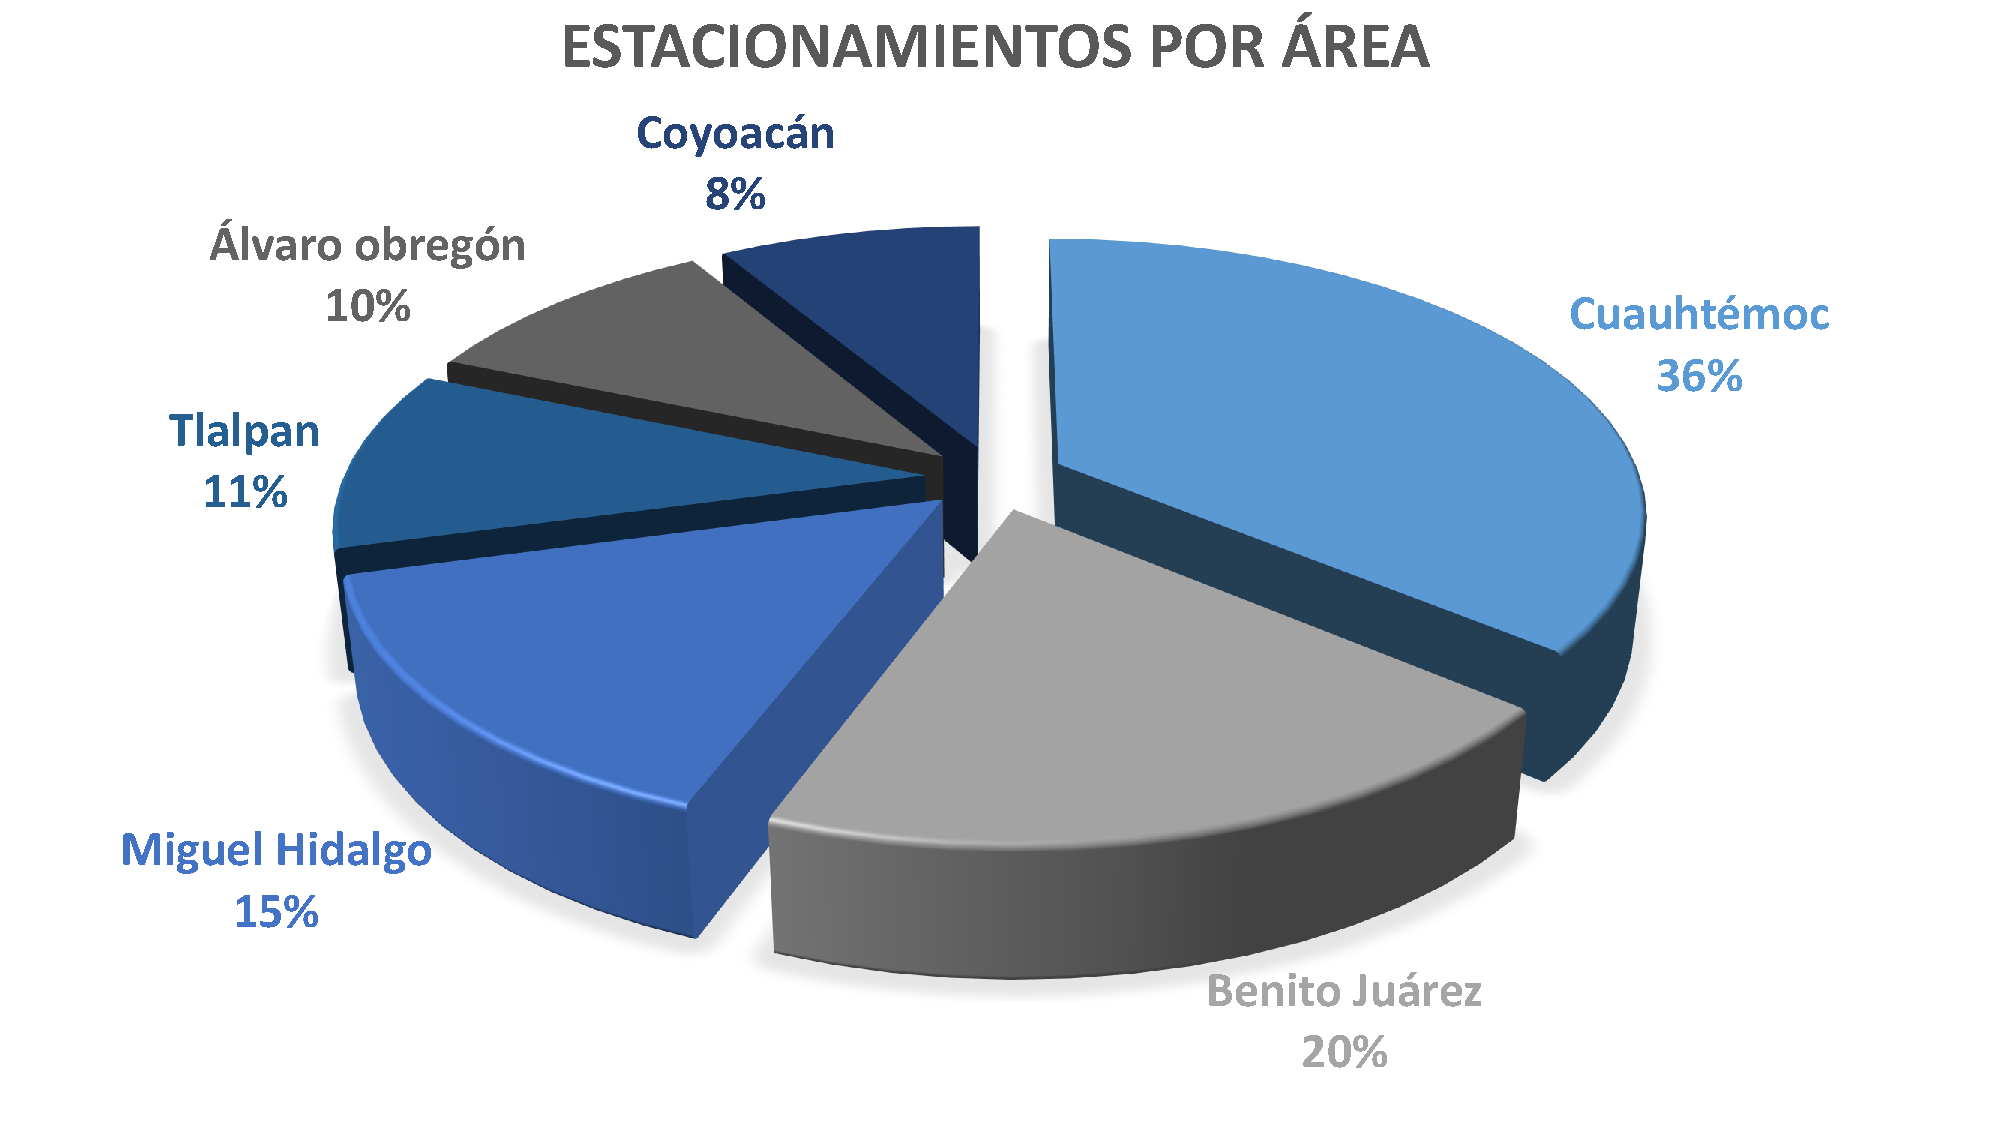
\includegraphics[scale=.3]{./analisisDeLaDemanda/source/estacionamientosPorArea}
	\caption{Estacionamientos por �rea en el DF}
	\label{fig:graficaEstacionamientosPorArea}
\end{figure}


Otra opci�n para estacionar en veh�culo es el parqu�metro, datos obtenidos a trav�s de ecoParq \cite{ecoparq}, hay 1,229 parqu�metros instalados, atendiendo a 19,890 cajones en la v�a publica, distribuidos de la como se muestra en el Cuadro \ref{tab:Parquimetros}.

\begin{table}[h]
	\centering
	\begin{tabular}{|l|c|c|}
		\hline COLONIA & PARQUIMETRO & CAJONES \\ 
		\hline Anzures & 113 & 1695 \\ 
		\hline Lomas-Virreyes & 162 & 3250 \\ 
		\hline Nochebuena & 32 & 500 \\ 
		\hline Polanco & 416 & 6240 \\ 
		\hline Roma/Condesa & 353 & 5535 \\ 
		\hline Florencia & 85 & 1470 \\ 
		\hline Ciudad de los deportes & 40 & 760 \\ 
		\hline Cr�dito - Constructor & 28 & 440 \\ 
		\hline
	\end{tabular}
	\label{tab:Parquimetros}
	\caption{Parquimetros y cajones por Colonia.}
\end{table}


Tomando como ejemplo la delegaci�n Cuauht�moc s�lo el 12\% de los autom�viles utilizan los aparcamientos p�blicos, mientras que 57\% aloja su veh�culo en estacionamientos privados, otro 28\% se estaciona en la v�a p�blica y s�lo 3\% de la poblaci�n lo hace en garaje propio \cite{autobild}.

\begin{figure}[h]
	\centering
	\includegraphics[scale=.3]{./analisisDeLaDemanda/source/TiposDeAlojamiento}
	\caption{Tipos de alojamiento, Delegacion Cuauht�moc}
	\label{fig:tiposDeAlojamiento}
\end{figure}


\subsection{CONSUMIDORES INDIRECTOS}
Consideramos a los consumidores indirecots como los usuarios que har�n uso del estacionamiento(usuarios finales). Seg�n datos del INEGI la flota  vehicular  registrada  en  el M�xico Distrito Federal se estima en 36.7 millones de veh�culos. \cite{INEGI}. En la Figura \ref{fig:vehiculosPorAno} podemos observar la cantidad de veh�culos y su tipo, asi como, el crecimiento que han tenido a�o con a�o desde 2003. 

\begin{figure}[h]
	\centering
	\includegraphics[scale=.5]{./analisisDeLaDemanda/source/VehiculosPorAno}
	\caption{N�mero de veh�culos por a�o seg�n su clase. Cifra mostrada en cientos de miles}
	\label{fig:vehiculosPorAno}
\end{figure}

El tipo de demanda que se detecta es insatisfecha, ya que, la gran mayor�a  de los estacionamientos (peque�os y medianos) opera solo con un dispositivo \textit{checador} que utilizan para contar el tiempo dentro del estacionamiento, y un registro  donde llevan el control de pensionados, y el total de las entradas. Figura \ref{fig:EstacionamientoChicoCompleto}.
\\
\begin{figure}
	\centering
  	\subfloat[Estacionamiento]{
   		\label{fig:Estacionamiento}
    	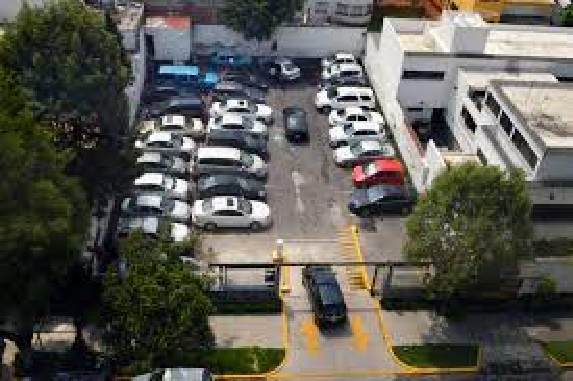
\includegraphics[width=0.3\textwidth]{./analisisDeLaDemanda/source/estacionamientoPequeno.pdf}
    }
  	\subfloat[Checador]{
   		\label{fig:relojChecador}
    	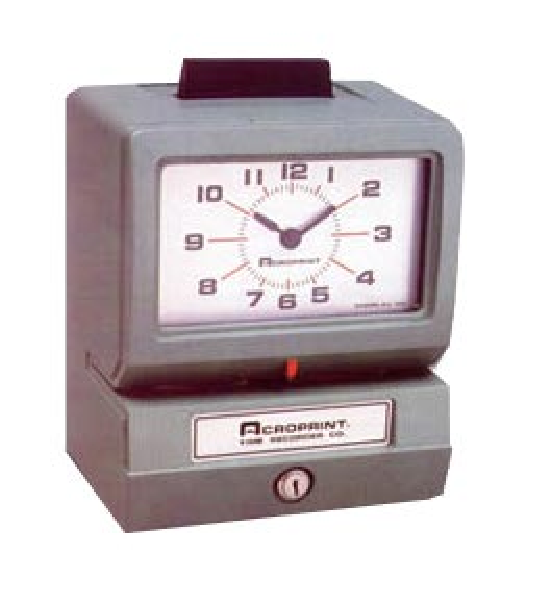
\includegraphics[width=0.15\textwidth]{./analisisDeLaDemanda/source/relojChecador.pdf}
    }
  	\subfloat[Conejo]{
   		\label{fig:libreta}
    	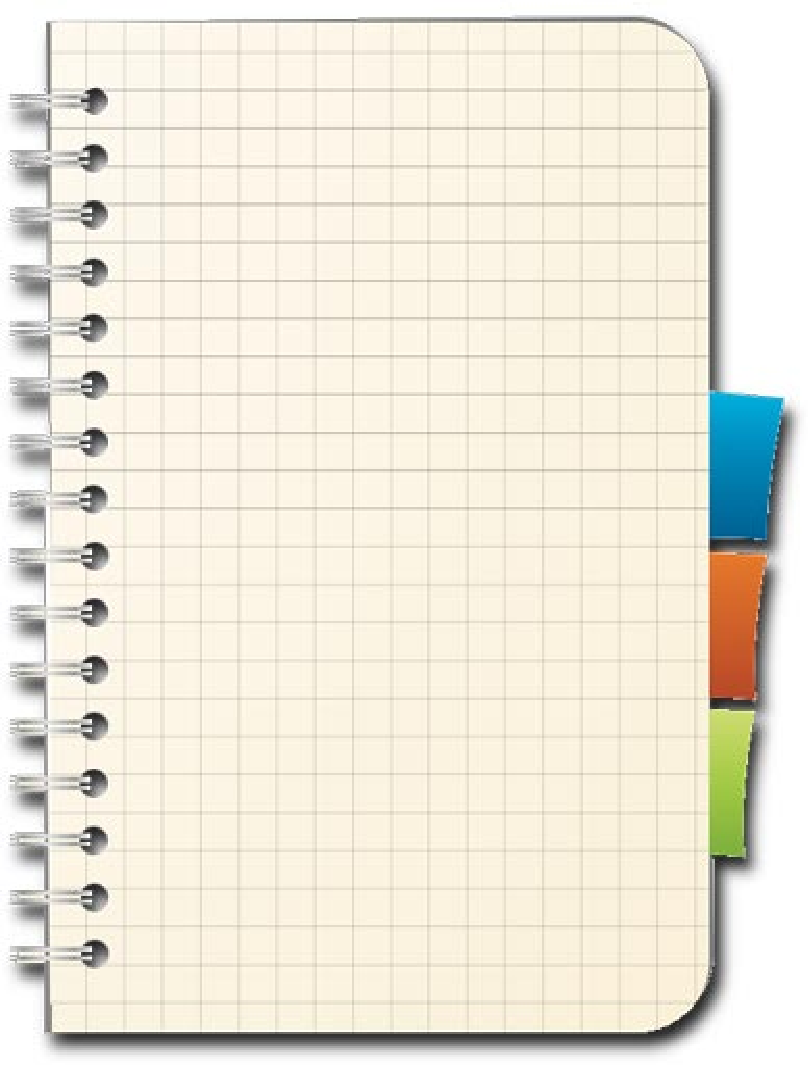
\includegraphics[width=0.15\textwidth]{./analisisDeLaDemanda/source/libreta.pdf}
    }
 	\caption{Estacionamiento chico y principales componentes}
 	\label{fig:EstacionamientoChicoCompleto}
\end{figure}

%SAE se enfoca en los estacionamientos peque�os y medianos ya que ellos representan un gran segmento del mercado y %resulta muy favorable para el ellos el uso de SAE (GANAR-GANAR).

Existen otro tipo de estacionamientos, estos los podemos encontrar en centros comerciales, plazas, s�per mercados, cines, teatros, zonas, hospitales, etc. Estos estacionamientos los definimos con \textit{estacionamientos grandes}. Estos tienen la caracter�stica de tener mayores ingresos y por ende poseen una mejor infraestructura. Figura \ref{fig:EstacionamientoGrandeCompleto}. Usualmente son administrador por un tercero y tiene sistema que automatiza las tareas operativas.  La desventaja principal de este tipo de estacionamientos es que el due�o del estacionamiento pierde el control del mismo y sus ingresos son   reducidos en gran medida, hasta de un 50\% de total, siempre y cuando el tercero haya recuperada la inversi�n inicial echa.  
Este tipo de estacionamientos no es nuestro principal cliente, pues ya posee un grado de automatizaci�n mayor; sin embargo SAE API brinda un conjunto de m�todos que pueden utilizar los sistemas externos para hacer uso de la plataforma que brinda SAE y con ellos aprovechar las ventajas que este brinda.


\begin{figure}
	\centering
  	\subfloat[modulodeCobro]{
   		\label{fig:EstacionamientoGrande}
    	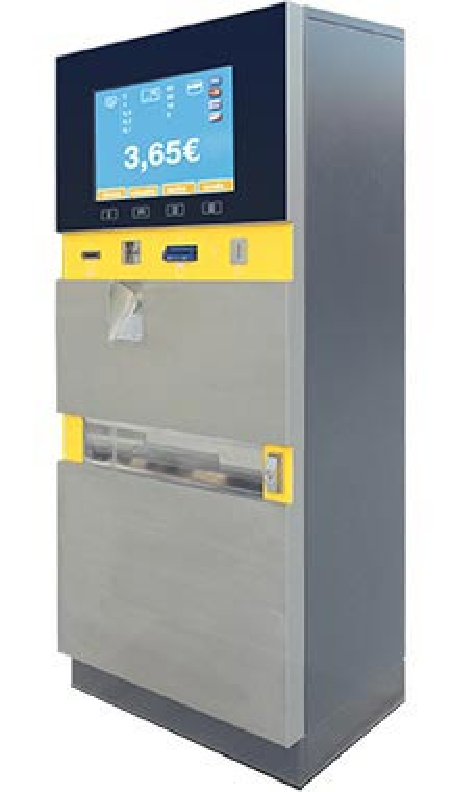
\includegraphics[width=0.23\textwidth]{./analisisDeLaDemanda/source/mouloDeCobro.pdf}
    }
  	\subfloat[pluma]{
   		\label{fig:pluma}
    	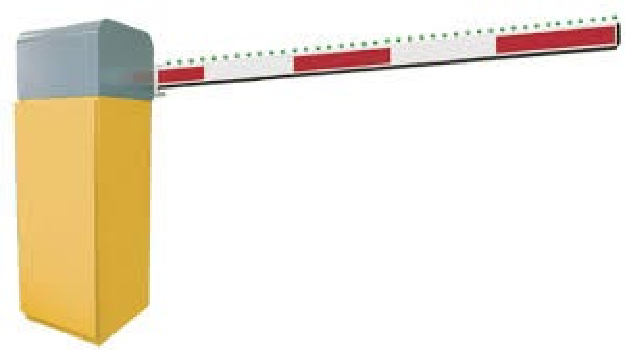
\includegraphics[width=0.5\textwidth]{./analisisDeLaDemanda/source/pluma.pdf}
    }
  	\subfloat[boletera]{
   		\label{fig:boletera}
    	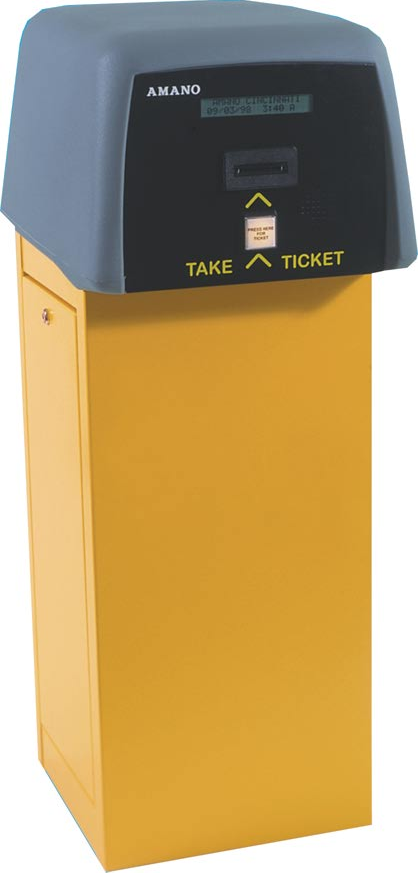
\includegraphics[width=0.14\textwidth]{./analisisDeLaDemanda/source/boletera.pdf}
    }
 	\caption{Infraestructura de estacionamientos grandes}
 	\label{fig:EstacionamientoGrandeCompleto}
\end{figure}

\newpage


		\section{An�lisis De La Oferta}
			\subsection{Soluciones para Administradores}
A continuaci�n se enlista las principales soluciones en el mercado para de la automatizaci�n y administraci�n de estacionamientos (software y hardware).

	\subsubsection{idPark}
		\input{./analisisDeLaOferta/idPark}
	\subsubsection{AVPM}
		\subsubsection{Nombre de la Empresa}
	AVPM

\subsubsection{Marca}
	AVPM
	
\subsubsection{Logo}
	\begin{figure}[ht]
		\centering
		
\includegraphics[scale=1]{./analisisDeLaOferta/source/logo_avpm}
		\caption{Logo AVPM}
		\label{fig:logo_avpm}
	\end{figure}

\subsubsection{Producto}
	AVPM provides Parking, Valet Parking and Bell desk solutions for different Market types. These solutions include Software, Hardware, consulting, implementation and support.
	
	We always use the latest technology on our software and hardware solutions. It does not matter how big or how small the project is, we use our expertise, our technology to deliver the best possible solution.
	
	We are well known to deliver the most innovative solutions to any project within the budget. We are well aware that no project could be the same as the previous one. We customize our system to the project specifics and make sure the system will work very efficiently at the location.



\subsubsection{Descripci�n}
	
	Automated Valet� is proud of the innovative solutions that we brought up to this industry. We use latest software and hardware solutions and combine them with our innovative approach to solve the most common problems very easily.
	Our system is highly scalable; you can start using one single handheld device (iPhone/ iPod/ handheld computer) or a point-of-sale computer and add garage access control devices, cameras, more computers and more handheld devices. We can host the system in our Cloud services or install the server on site, it is totally up to you!	
	We can offer you purchase, lease, month-to-month payment options depending on your hardware and software setup.
	
	\paragraph{AVPM� Touch Screen Interface}
		All of AVPM� applications come with a touch screen interface. AVPM� is a very user friendly system allowing end users to use the system without keyboard or mouse.
		
	\paragraph*{Q'd Up� Bell-desk/Valet Systems}
		Geolocation based task management queuing system for Bell Desk and Valet operations. Track everything from a guest?s luggage to flower delivery and closely monitor the steps of each employee based on their location on the property. Q?d Up� uses all this information to create a queue of tasks and assign them to each team members based on their availability.
	
	\paragraph*{AVPM� Operation Board Monitoring}	
		AVPM Operation Board MonitoringThis is an electronic monitoring system for your location. On Site or off site you will have access to this information and keep track of all of your employees, keys, cars, and garage. Every time a new transaction occurs, it gets recorded with a time stamp and different color.
	
	\paragraph{AVPM� TIS Ticket Inventory System}
		AVPM TIS Ticket Inventory SystemEvery missing ticket is lost revenue. AVPM� Ticket Inventory System is a crucial application to keep track of all your tickets and your revenue. With AVPM� TIS, tickets cannot be reused or duplicated, any ticket out of inventory will not be recognized by the system and cannot be used.
	
	\paragraph{AVPM� Fee Calculator/Rate Table}
		With AVPM� System, you do not need to call us to change rates. AVPM� System offers unlimited flexible rate structures that can be easily changed by the end user (an approved administrator). No more requesting rate changes and waiting for approvals!
	
	\paragraph{AVPM� Report Engine}
		AVPM Report EngineAVPM� offers over 100 different reports, no extra fees for any specialized reports. And if you do not see the report you like, we will create it for you at no charge! Most of AVPM� reports come in full color graphics, easy to run, and easy to understand. All reports can be exported to excel format and can be e-mailed.
	
	\paragraph{AVPM� Lost Key Warning System}
		AVPM Lost Key Warning SystemMonitoring of all keys will allow you to know where they are at all times. In the event of a misplaced key, the manager will know immediately.
	
	\paragraph{AVPM� Cashier\/Dispatcher Application}
		AVPM Cashier\/Dispatcher ApplicationWith AVPM� system end users will have immediate access to cashier and dispatcher applications on the main screen. They will be able to look up vehicles, search vehicles by any combination of yr, make, model, color, customer name, last name, and arrival time, employee who received the car or parked the car, room number, and license plate number.
	
	\paragraph{AVPM� Time \& Attendance}
		AVPM Time \& AttendanceWith AVPM� Time and Attendance we guarantee 20\% savings on your payroll! We recommend biometrics finger print technology for your employee clocking in and out purposes (additional finger print reader required). All employees will be required to use their finger print to clock in and out. Username, password and face identification (requires an additional camera) options available for AVPM� Time and attendance.
	
	\paragraph{AVPM� Payroll Interface}
		AVPM Payroll InterfaceAVPM� is capable of taking your employees clock-in and out times to create a ?time card? for payroll. It is also capable of computing the time into a readable format if your company is currently using a payroll system.
	
	\paragraph{AVPM� Credit Card Interface}
		AVPM Credit Card InterfaceAVPM� system has an integrated credit card solution and it is a PCI compliant system and a company. With the credit card interface valet locations can accept credit card payment from the system with no additional equipment other than an integrated, built in swipe card reader.
	
	\paragraph{PCI PA-DSS Compliance}
		Financial and personal information stored or processed through AVPM� is secure. It guarantees data security and prevents fraud. AVPM� meets the requirements set by the PCI Security Council for the safe storage and transfer of credit information regardless of venue.
	
	\paragraph{AVPM� VATS}
		AVPM VATSValidation Tracking System- Validation misuse will be totally avoided by using this feature which will generate scrambled letters and number bar-coded stickers that cannot be reused or duplicated. VATS are printed right from the AVPM� system, they have pre-printed expiration dates and can be easily voided in the system if lost.
		As an option we also offer online validation systems.
	
	\paragraph{AVPM� VATS+}
		AVPM VATS+Discount Coupon Program- Use your AVPM� system to create coupons for preferred customers and loyalty programs without jeopardizing revenue control. Create reusable validations where the expiration dates can be pre-selected so that VATS will only work on the right dates.
	
	\paragraph{AVPM� Enterprise}
		AVPM EnterpriseRemote monitoring system allows you to see what is going on at your location in real time from anywhere in the world. Real time reports are also available from remote locations using our Enterprise Software Solution. This also allows you to log into any of your locations if you have more than one using the AVPM� system.
	
	\paragraph{AVPM� VDES}
		AVPM VDESProDoor Interface- AVPM� software will decode VIN number and create VIN recognition through barcode scanning. Information relayed to the computer will include vehicle year, make and model, color, damage, and reservations. Keep up with who received the vehicle, who is parking the vehicle etc. set up email/text alerts to administrators to let them know when you have a VIP arriving with our VIP Recognition. With use of our Bluetooth scanners no information is ever lost and never needs to be re-entered from a computer.
	
	\paragraph{AVPM� ACCESS}
		AVPM ACCESSEmail/Text Message Request- Guests can request their vehicle from a remote location by sending a text message or an email to the system using their cell phones. The system will send a visual and written request to wherever your keys are stored for proper pick up.
	
	\paragraph{AVPM� Claim Tracking}
		AVPM Claim TrackingEasy to use and fill out, incident reports right from your AVPM� system. Pictures can be uploaded easily, and keeping track of the claim is simple. Corporate office can have this information with AVPM� Enterprise immediately.
	
	\paragraph{AVPM� Telephone Request Module}
		AVPM Telephone Request ModuleCustomers can call the system and request their cars by entering their ticket number on their phone. The telephone request module is just another way of making things more convenient for the customer.
	
	\paragraph{AVPM� Scheduler}
		AVPM SchedulerAVPM� System has a scheduler program that is built in, and can adapt to your locations scheduling needs. Schedules can also be emailed to employees from the system.
	
	\paragraph{AVPM� Garage Map Feature}
		AVPM Garage Map FeatureLocations that ?stack? their cars will be able to know when a car is blocking the requested vehicle and will be warned to pull both sets of keys. The system will also track the re-park location.
	
	\paragraph{AVPM� Valet Request Customer Display}
		AVPM Valet Request Customer DisplayAll transactions including arrivals and departures will be displayed on this unit. Every minute displays a different color with time stamp. Status of each vehicle and key will show with a time counter and different color.
	
	\paragraph{AVPM� License Plate Recognition System}
		AVPM License Plate Recognition SoftwareAVPM is proud to have in house LPR system. LPR system is designed to decode the numbers and letters from the license plates so the repeat, VIP customers can be identified instantly. Please see our VIN recognition/ decoding system for more VIP recognition options.
	
	\paragraph{AVPM� Frequent Parker Program}
		The frequent parker program keeps track of returning customers and can be setup to reward these frequent parkers with different promotions and discounts.
	
	\paragraph{AVPM� Garage Access Module}
		AVPM Garage Access ModuleGarage access control unit checks to make sure that it is a valid driver and it is a valid ticket (a ticket from the inventory), then grants the access. In the event that the ticket is not valid or the driver is not, the driver will not be able to go through the gates.
	
	\paragraph{AVPM� Vehicle Request Web Page/System Upgrade}
		AVPM Vehicle Request Web Page/System UpgradeCustomers will be able to request their vehicles in their room when checking out from the web enabled TV.
	
	\paragraph{AVPM� Hotel Management System Interface}
		AVPM Hotel Management System InterfaceInterface with Hotel Management Systems to post overnight charges to rooms and post transient guest charges to a room automatically, saving you revenue.
	
	\paragraph{AVPM� Room Key Interface}
		AVPM Room Key InterfaceAVPM� system will be able to collect information such as room number, first name and last name, insert it to the valet ticket when swiped to the system. Customers can also request their vehicles with this integration.
	
	\paragraph{AVPM� Front Desk Manager}
		AVPM Front Desk ManagerAVPM� Front Desk Manager is designed to enter guest information by Front Desk Employees to AVPM� system. Depending on the Hotel Management system used, AVPM� will be able to automatically post the parking fees to the guest folios. Required fields can be different on different interfaces. It is also designed to request vehicles. Vehicles can be requested by entering valet ticket number or room number if it is entered to the system.
	
	\paragraph{AVPM� Players Card Integration}
		AVPM Players Card IntegrationAVPM� is capable of integrating with Casino Player?s cards, to recognize VIP?s, add points, and request their vehicle. (Cards Mag-stripe required).
	
	\paragraph{AVPM� Flight Database Integration}
		AVPM Flight Database IntegrationThis integration with a real time flight database will track when customer?s flights are coming in, late or cancelled. The system pulls only the related customer information including gate and luggage arrival. This feature is available and recommended for all airport (On or off-site) locations.
	
	\paragraph{AVPM� Reservation Page Valet Boarding Pass}
		AVPM Reservation Page Valet Boarding PassThis integration with your current website will create a link to a ?Reservation page? allowing your customer to go online, make a reservation, and print out a Valet Boarding Pass with barcodes. It is integrated with AVPM� database, so when receiving the car the valet will scan the barcodes from the Valet Boarding Pass and all applicable information on the driver and vehicle (year/make/model/airline) will attach itself to the ticket automatically. This feature is available and recommended for all airport (On or off-site) locations.
	
	\paragraph{AVPM� Staging Board}
		AVPM Staging BoardAdditional Monitoring Board working with your flight database integration to display arrivals, departures, baggage area location, gate location and delays daily, of all of your returning customers.
	
\subsubsection{Precio}

\subsubsection{Pa�ses donde se comercializa}
	EUA

\subsubsection{Otros Datos}

\subsubsection{Link}
	\url{http://automatedvalet.com/}
	\subsubsection{EQUINSA PARKING}
		\paragraph{Nombre de la Empresa}
	SENSE-Parking solution

\paragraph{Marca}
	EQUINSA PARKING
	
\paragraph{Logo}
	Figura \ref{fig:logoEquinsaParking}
	\begin{figure}[h]
		\centering
		
\includegraphics[scale=.7]{./analisisDeLaOferta/source/logoEquinsaParking}
		\caption{Logo EquinsaParking}
		\label{fig:logoEquinsaParking}
	\end{figure}

\paragraph{Producto}
	Gesti�n y Administraci�n de Estacionamientos

\paragraph{Descripci�n}
	\subparagraph{Software de Gesti�n} 
			
		Software modular, abierto y adaptable. La premisa fundamental del dise�o del software de gesti�n del sistema Sense de Equinsa, adem�s de su fiabilidad, es su adaptabilidad. 
		
		Ha sido concebido con la idea de la m�xima reutilizaci�n, de manera que gran parte de los m�dulos de gesti�n y comunicaciones son comunes para todos los elementos del sistema. Esto permite simplificar en gran manera los procedimientos de mantenimiento y actualizaci�n del software, y los hace m�s robustos.
	
			
		Con el Sistema Abierto de Operaci�n y Control SENSE  se pueden configurar diferentes puestos de operador de acuerdo con las necesidades y tipo de explotaci�n del aparcamiento porque est�  concebido mediante M�dulos Software. que  se instalan en arquitecturas PC  (donde siempre existir� el m�dulo Servidor )  al objeto de configurar cualquier tipo de Puesto de Operador como indican las configuraciones referidas a continuaci�n:
		
		\begin{itemize}
			\item Configuraci�n con un �nico PC
			\item Configuraci�n con dos PCs (Puesto de Cobro/Supervisi�n separado )
			\item Configuraci�n con varios puestos de Cobro/Supervisi�n
			\item Configuraci�n de varios puestos con funcionalidades iguales o diferentes
			\item Configuraci�n simplificada con el Terminal SENSE - EA2 CC
			\item Como queda dicho, el software  esta ideado para su  utilizaci�n en arquitectura PC con sistema operativo Windows. Hemos \item elegido esta opci�n puesto que Windows es el sistema operativo m�s ampliamente implantado, y su presencia es universal, lo que garantiza que un gran n�mero de usuarios est�n familiarizados con su aspecto y uso, como m�nimo a nivel de usuario.
		\end{itemize}
		
		Asimismo, utiliza  SQL Server como gestor de BBDD. La calidad, robustez y prestaciones de Microsoft SQL Server est� fuera de toda duda, y aporta a nuestro sistema grandes posibilidades tanto a nivel de operativa como de integridad de datos.
		
		El men� de operaci�n es muy intuitivo y amigable, permitiendo al operador realizar c�modamente las operaciones de Cobro y Supervisi�n y al explotador tener total control del sistema, as� como la obtenci�n en tiempo real de toda la informaci�n relevante que aporta:
		
		\begin{itemize}
			\item Datos contables 
			\item Estad�sticas 
			\item Incidencias 
			\item Listados
			\item El sistema permite ser utilizado por m�ltiples usuarios con distintos permisos de acceso, quedando as� protegidos determinados datos y su manipulaci�n indebida.
		\end{itemize}
		
		Su potente software de gesti�n permite la realizaci�n de todo tipo de estad�sticas tales como ingresos, ocupaci�n, estancias, horas punta, etc.
		
		Asimismo, incluye la capacidad de Telegesti�n via red local o internet, por la que pueden establecerse puestos remotizados para tareas de Gesti�n, Diagn�stico, Parametrizaci�n?
	
	\subparagraph{Software de Matr�culas}	
		
		El sistema de Control de Matr�culas ha sido desarrollado para ofrecer al explotador una potente herramienta de ayuda al sistema de gesti�n que puede ser instalado independiente o en conjunto con el sistema de gesti�n de Equinsa Parking. El sistema es muy �gil y r�pido a nivel de v�as, de manera que los usuarios no notar�n su presencia (la salida del ticket no se demorar�). Adem�s de la matr�cula, el sistema permite la captura de im�genes laterales del veh�culo e incluso una imagen facial del conductor, que el explotador podr� cotejar en caso de incidencias o problemas en el aparcamiento.
		
		Potentes herramientas de explotaci�n y gesti�n permitir�n la b�squeda y la emisi�n de informes de manera complementaria a los del propio sistema de gesti�n del aparcamiento que redundar�n en un superior control de determinadas incidencias dentro del mismo.
		
		El Sistema de Control de Accesos RAMA constituye una soluci�n en recintos de aparcamiento que permite la entrada y salida de veh�culos mediante el control realizado sobre la matr�cula reconocida tanto en entrada como en salida. Trabaja con usuarios dados de alta en el Sistema (Base de Datos).
		
		El sistema permite adem�s definir zonas, as� como contadores en las mismas, aportando una gran flexibilidad en las posibles acciones a tomar de acuerdo con el estado de los contadores establecidos. Uno de los valores a�adidos del sistema adem�s del control, es el perfil de seguridad que aporta.
		
		En el sistema se distinguen los siguientes elementos:
	
	\subparagraph{ 1.- Subsistema RAMA}
		Controla todos los perif�ricos de acceso y el reconocimiento de matr�culas mediante el motor RAMA y las c�maras correspondientes. Se ubica en las entradas/salidas y se instalar�n tantos cuantos resulten necesarios, en funci�n del n�mero de entradas y salidas del recinto. Todos ellos est�n conectados v�a Ethernet con el puesto donde se instale la Base de Datos y la Aplicaci�n Gestor. Funciones:
		\begin{itemize}
			\item Alta de abonados y empresas.
			\item Creaci�n de zonas.
			\item Configuraci�n del sistema.
			\item Vista de m�quinas.
			\item Obtenci�n de listados.
			\item En el alta de abonados pueden asociarse a una �nica plaza varias matr�culas.
			\item En la vista de m�quinas se permite la se�alizaci�n de incidencias en las v�as.
		\end{itemize}
	
	
	\subparagraph{2.- Base de Datos}
		Constituye el medio de almacenamiento y consulta de toda la informaci�n necesaria para el funcionamiento del sistema. Se puede  actualizar datos en la Base de Datos y obtener Listados. Funciones para abonados, tarifas, empresas y usuarios:
		\begin{itemize}
			\item Altas.
			\item Bajas.
			\item Modificaciones de datos.
			\item A�adir matr�culas.
			\item Antipassback.
			\item Se ofrecen m�ltiples listados sobre abonados, empresas? y movimientos.
		\end{itemize}
	
	\subparagraph{Software de Guiado}
		Los sistemas de Guiado de Equinsa Parking se basan en la detecci�n de objetos por medio de sondas de ultrasonidos que emiten y reciben en una frecuencia de 4KHz.
		
		Estas sondas est�n alojadas junto con la electr�nica de control de cada unidad en una caja espec�ficamente dise�ada para tal fin y deben ser colocadas en el techo (en el centro de la plaza  o en el pasillo dependiendo de que modelo se seleccione) dentro de un rango de altura que viene indicado en las especificaciones T�cnicas.
		
		Estas sondas pueden ir equipadas con unos diodos emisores de luz que cambian de color en funci�n de la ocupaci�n de la plaza, pasando del estado de plaza vac�a = Verde al de plaza ocupada= Rojo. Tambi�n existe la opci�n Azul = Plaza para Minusv�lido  Las diferentes soluciones se aplican en funci�n de la existencia o no, de columnas que dificulten la visi�n de la se�alizaci�n.
		
		El sistema se complementa con una serie de carteles luminosos colocados en las intersecciones de los viales,  que indican mediante un grafismo de flechas y aspas rojas y verdes y sus correspondientes d�gitos a Led, el n�mero de plazas disponibles en cada zona del aparcamiento o en el resto de las plantas.
		
		Todo ello queda recogido y controlado desde un programa que suele  instalarse en un ordenador espec�fico aunque igualmente puede ser instalado en el Ordenador central del estacionamiento.
		
		Los sistemas  GUIA (Gesti�n de Usuarios en el Interior del Aparcamiento) de Equinsa Parking, en sus dos versiones de  sonda mas extensi�n y ?todo en uno?, mediante su potente software de operaci�n  permiten al operador obtener las siguientes prestaciones:  
		
		\begin{itemize}
			\item Detecci�n de la ocupaci�n de las plazas en el aparcamiento mediante sondas de ultrasonidos.
			\item Se�alizaci�n del estado de cada plaza con la opci�n de cambio de estado desde el sistema.
			\item Guiado de veh�culos en el interior del aparcamiento mediante carteles de informaci�n al usuario
			\item Registro inform�tico del estado de ocupaci�n del aparcamiento.
		\end{itemize}
		
		Los carteles indicadores informan al usuario de la disponibilidad de plazas libres y les gu�an hasta ellas, indicando el n�mero de plazas disponibles as� como su ubicaci�n dentro del aparcamiento mediante un completo sistema de flechas y aspas.
		
		Este sistema proporciona al operador  entre otras  herramientas, estad�sticas de nivel de ocupaci�n,  generaci�n autom�tica de listados de plazas con tiempos superiores al umbral determinado por el gestor y listados autom�ticos de veh�culos estacionados a partir de una hora determinada por el gestor, lo cual facilita la toma de datos por parte del servicio de seguridad del aparcamiento, As� mismo puede bloquear desde el PC las plazas a ocupado y libre, permitiendo aparcar los veh�culos por zonas con el consiguiente ahorro energ�tico de las zonas no ocupadas cuando la demanda de plazas as� lo aconseje. Adem�s incrementa notablemente el rendimiento del estacionamiento en momentos de m�xima ocupaci�n al liberar la plaza en el momento en que un auto la abandona sin necesidad de esperar a que cruce por la barrera de salida para darle el nivel ?Libre?.. Tambi�n permite  evaluar el impacto de ocupaci�n  puntual mediante  la parametrizaci�n previa del nivel de ocupaci�n esperado.
		
		Finalmente, este novedoso concepto de aparcamiento mejora la calidad de servicio ofrecido al usuario, permitiendo aparcar en menor tiempo, y disminuyendo el nivel de contaminaci�n.
	
	\subparagraph{Valet Parking}
	
	El m�dulo VALET EQUINSA permite la gesti�n de zonas destinadas al servicio de aparcamiento VALET con sistemas Sense. Con este m�dulo de aparcamiento conseguiremos agilizar considerablemente la entrada  y salida de veh�culos en el recinto, lo cual repercutir� favorablemente tanto al cliente,evitando esperas innecesarias en busca de una plaza, como al parking,optimizando las plazas libres.
	
	Prestaciones Valet Parking
	Requisitos
	Requisitos
	
	El sistema estar� compuesto por:
	
	
	\begin{itemize}
		\item Sistema de Gesti�n de parking Sense.
		\item Conexi�n inal�mbrica con acceso al servidor Sense.
		\item Dispositivo port�til con sistema operativo Android 4.0 o superior (Tablet) con acceso a la red inal�mbrica.
		\item Impresora de tickets port�til Bluetooth o Wifi.
		\item Zona de recepci�n de los veh�culos.
		\item Zona de devoluci�n con PC, Impresora de tickets y lector de tarjetas mifare.
		\item Modo de operaci�n
	\end{itemize}
	
	El funcionamiento b�sico se inicia con la entrega de las llaves del veh�culo por parte del cliente al personal del parking ubicado en la zona destinada a tal uso. 
	Con la ayuda de un dispositivo m�vil e impresora, que facilitar� el movimiento del personal por la zona,el cliente recibir� un ticket que almacena los datos necesarios para realizar el posterior pago en caja.
	
	
	El encargado de registrar la entrada del veh�culo asignar� a �ste: 
	
	\begin{itemize}
		\item 	Un identificador(objeto visible para facilitar la recogida, plaza, zona, etc.).
		\item	Matr�cula y fotos del estado en la entrada. En caso de disponer del sistema de reconocimiento autom�tico de Matr�culas (RAMA) se podr� consultar la lista de lo �ltimos veh�culos que entraron. Si no fuera as� la introducci�n ser� manual.
		\item	Marca del veh�culo.
		\item Modelo y color.
		\item	Objetos depositados en el interior del veh�culo.
		\item	Una vez realizado el ingreso de los datos se proceder� al aparcamiento del veh�culo.
	\end{itemize}

	
	Este proceso puede realizarse en paralelo para agilizar en la medida de lo necesario el movimiento de los veh�culos.
	
	Una vez que el cliente decide terminar su estancia y realiza el pago en cualquiera de las cajas habilitadas el sistema se encargar� autom�ticamente de iniciar el proceso de devoluci�n del veh�culo.
	
	Para ello, el sistema cuenta con un PC en la zona habilitada para esta operaci�n, que gestionar� la entrega. En la pantalla del mismo y por orden de pago aparecer� un listado con los veh�culos que est�n en proceso de ser entregados al cliente.
	
	
	Cada empleado apto para realizar la devoluci�n dispondr� de una tarjeta contactless que servir� para identificarse en dicho PC e iniciar el proceso de retorno del primer veh�culo situado en la lista mencionada con anterioridad. El sistema imprime un ticket con informaci�n sobre la identificaci�n del veh�culo que servir� al empleado para la localizaci�n del mismo.
	
	
	Una vez finalizado el proceso de entrega al cliente, el empleado volver� a identificarse para registrar la entrega del veh�culo.
	
	El sistema de valet parking the Equinsa es residente en el software de gesti�n del estacionamiento y esta integrado en el mismo por lo cual se beneficia de las prestaciones caracter�sticas del software general que permite la realizaci�n de todo tipo de estad�sticas tales como ingresos, ocupaci�n, estancias, horas punta, etc. As� como la obtenci�n de:
	
	\begin{itemize}
		\item Datos contables 
		\item Estad�sticas 
		\item Incidencias 
		\item Listados
	\end{itemize}

	El men� de operaci�n es muy intuitivo y amigable, permitiendo al operador realizar c�modamente las operaciones de Cobro y Supervisi�n y al explotador tener total control del sistema, as� como la obtenci�n en tiempo real de toda la informaci�n relevante que aporta:
	
	El sistema permite ser utilizado por m�ltiples usuarios con distintos permisos de acceso, quedando as� protegidos determinados datos y su manipulaci�n indebida.
	
\paragraph{Precio}

\paragraph{Pa�ses donde se comercializa}
	\begin{itemize}
		\item M�xico
		\item Brasil
		\item Espa�a
		\item Portugal
		\item Puerto Rico
	\end{itemize}
	

%\paragraph{Otros Datos}

\paragraph{Link}
	\url{http://www.equinsaparking.com/es}
	\subsubsection{Smartpark Management Software}
		\paragraph{Nombre de la Empresa}
	TIBA PARKING LLC.

\paragraph{Marca}
	Smartpark Management Software	
\paragraph{Logo}
	Figura \ref{fig:logo_smartPark}
	\begin{figure}[ht]
		\centering
		
\includegraphics[scale=1]{./analisisDeLaOferta/source/logo_smartPark}
		\caption{Logo SmartPark }
		\label{fig:logo_smartPark}
	\end{figure}

\paragraph{Producto}
	Property owners and managers are looking for a facility management system that is reliable, feature
	rich, flexible and that does not require frequent and costly upgrades to remain operational. They are
	also looking for straight forward solutions to their operational challenges.
	
	TIBA Smartpark is the answer they\'ve been looking for! Whether your property is an office
	building, hotel, medical center or a mix-use development, Smartpark has the intelligent solutions
	custom tailored to manage these types of facilities. Smartpark is a scalable product from a single
	facility to an entire city parking system.

\paragraph{Descripci�n}
	\subparagraph{Monitoring and Control}
		 With Smartpark, operators can monitor and control all aspects of their facilities including occupancy, system alarms, VMS signs, equipment status, and lane traffic. They can also open/close barrier gates, restart lane equipment, or even send a new fee to a pay station. Additionally key facility personnel can receive email alerts and/or reports for virtually any system activity.
	
	\subparagraph{Revenue Management}
		Smartpark is your turn-key facility management solution including real time transactions, ticket tracking, occupancy counts, alarm monitoring, parking rate programming, coupons, validations, zone counts, sign controls and much more. From a single dashboard monitor system alarms, revenues transactions, equipment status, cardholder traffic, open tickets and facility occupancy. See it all locally, on the web and from your smartphone. Validation and coupon management and production is made simple cost effective with an integrated module that comes standard with Smartpark.
	
	\subparagraph{Validation Solutions}
		TIBA Smartpark offers a wide range of intelligent validation solutions. In Smartpark, merchant accounts and sub-accounts are created in the database. An unlimited amount of merchant accounts can be created in Smartpark. Additionally the validation types are created, i.e. one-hour free, \$1 discount. The validation types are created once and are available and can be utilized by any merchant account. After the validation profi les are created they are available for all applications including; barcode stickers, coupons (chaser tickets), QR codes, online desktop units, self-service units, off-line desktop units and for web client accounts.
		
	\subparagraph{Access Control}
		 Parking access today requires a wide range of controls and billing options that provide owners and facility managers the fl exible solutions to bring in new business. Smartpark is your enterprise parking access control solution. Whether it\'s a single, monthly contract account or an entire company, Smartpark provides intuitive access control management. Take advantage of the latest and greatest credential technologies such as LPR, AVI, QR and chip card, the choice is yours. Smartpark supports cardholder payments and value card re-charge at pay-on-foot stations in our standard product.

	\subparagraph{Standard Features}
		\begin{itemize}
			\item Debit/Value Card
			\item Tenant management
			\item Shared accounts
			\item Automatic-activation
			\item Corporate accounts
		\end{itemize}
	
	\subparagraph{Reporting}
		Smartpark provides a full complement of reports for all aspects of your facility including transient, monthly, valet, hotel, pre-paid and event activity. TIBA Smartpark provides real-time revenue reporting on a local and enterprise scale. Additionally Smartpark tracks hourly occupancy, entry/exit statistics, transient transactions and contract activity. All reports can be exported to excel, word, PDF, text files and other formats
	
\paragraph{Precio}

\paragraph{Pa�ses donde se comercializa}
	EUA
%\paragraph{Otros Datos}

\paragraph{Link}
	\url{http://www.tibaparking.com/smartpark-management-software-2/}
	\subsubsection{3M Parking Software}
		\subsubsection{Nombre de la Empresa}
	3M
\subsubsection{Marca}
	3M Parking Software
	
\subsubsection{Logo}
	\begin{figure}[ht]
		\centering
		
\includegraphics[scale=.2]{./analisisDeLaOferta/source/logo_3M}
		\caption{Logo 3M }
		\label{fig:logo_3M}
	\end{figure}

\subsubsection{Producto}
	Operational Excellence Starts with Software
	
\subsubsection{Descripci�n}
	A smarter, more data-driven software platform can drive your business toward top-tier performance and lasting operational excellence. 3M? Parking Enterprise Facility Management (FMS) Software is an open, interoperable and scalable software platform that is changing the parking industry. The scalable and modular architecture promotes integration, isolates services in a modular format and further simplifies development and upgrades. It even facilitates 3rd party application development, so you can easily use solutions from a variety of providers, and gain maximum flexibility in creating business rules that fit your operational design.
	
	3M parking software coalesces years of systems expertise into a first-class software architecture! Your user experience is specifically designed to turn raw data into useful, accessible information -- real-time results let you make real-time decisions!
	
	3M Enterprise FMS is a bold step forward in operational management, and we have only just begun. As we build more modules, hardware options and 3rd party interfaces onto the platform, you can be sure they will exhibit the same focused attention to delivering real world value that?s elementally different.
	
	See 3M Parking Solutions for more information about our 360-degree solutions that can be configured to meet unique application needs.
	
	Please contact us to purchase or learn more about 3M Parking Software.

\subsubsection{Precio}

\subsubsection{Pa�ses donde se comercializa}
	EUA
%\subsubsection{Otros Datos}

\subsubsection{Link}
	\url{http://solutions.3m.com/wps/portal/3M/en_US/NA_Motor_Vehicle_Services_Systems/Motor_Vehicle_Industry_Solutions/product_catalog/parking-tolling-and-dmv-vehicle-software-3m-motor-vehicle-systems/parking-software/}
	\subsubsection{Software Playas de Estacionamiento}
		\paragraph{Nombre de la Empresa}
	Grandi y Asociados
\paragraph{Marca}
	Software Playas de Estacionamiento
	
\paragraph{Logo}
	Figura \ref{fig:logo_Grandiyasociados}
	\begin{figure}[h]
		\centering
		
\includegraphics[scale=.6]{./analisisDeLaOferta/source/logo_Grandiyasociados}
		\caption{Logo Grandi Y Asociados}
		\label{fig:logo_Grandiyasociados}
	\end{figure}

\paragraph{Producto}
	Software Playas de Estacionamiento

\paragraph{Descripci�n}
	Gesti�n completa para playas de estacionamiento, con control de ingreso y salida de veh�culos. Diferentes categor�as y tarifas por fracci�n configurable, tarifas fijas, por abono. Tarifas especiales, aplicaci�n de descuentos. Control total sobre el estado de ocupaci�n de la playa. R�pido registro del ingreso vehicular y agilidad en el cobro y salida del veh�culo.
	Gesti�n de pagos mensuales mediante abonos, con registraci�n de veh�culos autorizados por abono.
	
	\paragraph{Caracter�sticas Funcionales	}
		\begin{itemize}
	
			\item Gesti�n de ingreso y salida de veh�culos utilizando solo el teclado.
			\item Teclas de funci�n programables desde sistema.
			\item Tipos de veh�culos configurables.
			\item Tarifario m�ltiple, permitiendo contar con tarifas especiales por tipo de veh�culo. Tarifas por hora, por fracciones configurables. 
			\item Tarifas fijas.
			\item Manejo de planes especiales o abonos, con asignaci�n de veh�culos autorizados.
			\item Res�menes diarios, semanales, mensuales de la ocupaci�n de playa, de veh�culos ingresados, de horas de estacionamiento utilizadas por veh�culo.
			\item Consultas configurables acorde a los requerimientos del cliente.
			\item Control de descuentos, bonificaciones, recargos y cambios de precios al facturar.
			\item M�ltiples turnos y cajeros.
			\item Cierre de caja con ingreso discriminado por tipo de veh�culo.
			\item Todos los m�dulos de gesti�n administrativa b�sicos: facturaci�n, compras, cuentas corrientes, caja, formas de pago, bancos, impuestos, Libro IVA Ventas y Compras, contabilidad integrada.
		\end{itemize}
		
	\paragraph{Caracter�sticas Operativas}
		\begin{itemize}
			\item Auto instalable.
			\item Puesta en marcha inmediata.
			\item Ayuda sensible al contexto en todas las opciones del programa.
			\item Multiusuario.
			\item Manejo de perfiles de usuario con asignaci�n de permisos.
			\item Asignaci�n de perfiles de acceso a las distintas opciones del men� por usuario y programa.
			\item Restricciones de acceso a los usuarios a determinada informaci�n a trav�s de las consultas.
			\item Se adapta a la impresora que usted utiliza.
			\item Definici�n de impresoras por puesto de trabajo y\o comprobante.
			\item Genera informes imprimibles o visualizados en la pantalla.
			\item Puede configurar en forma personalizada todos sus formularios.
			\item Generador de informes, reportes, consultas y listados definibles y personalizados.
			\item Enlace con Excel y exportaci�n de datos a otros sistemas.
			\item Informes y estad�sticas de utilizaci�n del sistema. Auditoria por Programa y Fecha, Auditoria por Usuario y Fecha.
		\end{itemize}
		
	\paragraph{Requerimientos}
		PC Plataforma Windows XP o superior. 2 Gb de RAM y disco r�gido de 120 GB. Puertos Series necesarios. Monitor con resoluci�n minima de 1024 x 768.

\paragraph{Precio}

\paragraph{Pa�ses donde se comercializa}
	M�xico
%\paragraph{Otros Datos}

\paragraph{Link}
	\url{http://www.grandiyasociados.com.ar/software.asp?IDSoftware=9}	
	\subsubsection{Resumen}
		El Cuadro muestra un resumen con las principales caracter�sticas de las soluciones
\\
\begin{center}
\rowcolors{2}{grisClaro}{white}

\begin{tabular}{|l|c|c|c|c|c|c|}
	\hline  & idpark & Automated Valet & EQUINSA PARKING & Smartpark & 3M Parking Software & Software Playas de Estacionamiento \\\hline 
	Estacionamientos & \checkmark & \checkmark & \checkmark & \checkmark & \checkmark & \checkmark \\\hline 
	Pension& \checkmark &  &  &  &  &  \\\hline 
 	Valet &  & \checkmark & \checkmark &  &  &  \\\hline
 	Control de entradas\/salidas & \checkmark & \checkmark & \checkmark & \checkmark & \checkmark & \checkmark \\\hline
 	Corte de caja & \checkmark &  &  &  &  &  \\\hline
 	Clientes preferentes & \checkmark & \checkmark &  &  &  &  \\\hline
 	Tarifas configurables & \checkmark & \checkmark & \checkmark & \checkmark & \checkmark & \checkmark \\\hline 
 	Boleto perdido & \checkmark &  &  &  &  &  \\\hline 
 	Reportes & \checkmark & \checkmark & \checkmark & \checkmark & \checkmark & \checkmark \\\hline
 	Gelocaclizacion de valet &  &  & \checkmark &  &  &  \\\hline
 	Aletas &  & \checkmark &  & \checkmark &  &  \\\hline
 	Cuentas de usuario &  & \checkmark & \checkmark & \checkmark & \checkmark & \checkmark \\\hline 
 	Chat &  & \checkmark &  &  &  &  \\\hline
 	Facturaci�n &  &  &  & \checkmark &  &  \\\hline
 	Contabilidad &  &  &  &  &  & \checkmark \\\hline 
 	Multiples entradas/salidas & \checkmark &  & \checkmark &  &  &  \\\hline
 	%Pago &  &  &  &  &  &  \\\hline  
 	Unidad de cobro (HW) & \checkmark & \checkmark & \checkmark &  &  &  \\\hline  
 	Unidad de pre-pago manual (HW)  & \checkmark & \checkmark & \checkmark &  &  &\\\hline 
 	Pluma (HW) & \checkmark & \checkmark &  &  &  &  \\\hline 
 	Camara(HW) &  & \checkmark & \checkmark &  &  &  \\\hline  
 	Acceso con dispositivo (HW) & \checkmark &  &  & \checkmark &  &  \\\hline  
 	Punto de venta (HW) &  & \checkmark &  &  &  &  \\\hline  
 	Impresora (HW) & \checkmark & \checkmark & \checkmark & \checkmark & \checkmark & \checkmark \\\hline  
 	Terminar para tarjeta (HW) &  & \checkmark &  & \checkmark &  &  \\\hline  
 	Sistema de guiado (HW) &  &  & \checkmark &  &  &  \\\hline  
 	Carteles indicadores (HW) &  &  & \checkmark &  &  &  \\\hline  
 	Windows &  &  & \checkmark &  &  &  \\\hline  
 	Local &  & \checkmark & \checkmark &  & \checkmark & \checkmark \\\hline  
 	Online / Cloud Services & \checkmark & \checkmark &  & \checkmark &  &  \\\hline  
 	Reconocmiento de placa &  &  & \checkmark &  &  &  \\\hline 
\end{tabular} 
\end{center}
		
\subsection{Soluciones para Usuarios Finales}
A continuaci�n se enlista las principales soluciones en el mercado para de la locarilaz estacionamientos desde un smartphne. 

	\subsubsection{eTarifado}
		\paragraph{Logo}
	Figura \ref{fig:logo_eTarifado}
	\begin{figure}[h]
		\centering
		
\includegraphics[scale=.6]{./analisisDeLaOferta/source/logo_eTarifado}
		\caption{Logo eTarifado}
		\label{fig:logo_eTarifado}
	\end{figure}

\paragraph{Descripci�n}
eTarifado te permite enviar un SMS al servicio de estacionamiento tarifado de la IMM de una forma muy simple.
Olvida tener que buscar el quiosco m�s cercano para comprar 30 minutos de estacionamiento!
Con esta aplicaci�n vas a poder reservar el estacionamiento inmediatamente, sin errores al poner tu matricula ni el tiempo que quieras reservar.

\paragraph{Precio}
	Gratis

\paragraph{Plataformas}
	\begin{itemize}
		\item iOS
		\item Android
	\end{itemize}
	
\paragraph{Link}
	\begin{itemize}
		\item \url{https://itunes.apple.com/mx/app/etarifado/id579738553?mt=8}
		\item \url{https://play.google.com/store/apps/details?id=com.pagapp.etarifado&hl=es_419}
	\end{itemize}
			
	\subsubsection{Aparca Coches}
		\paragraph{Logo}
	Figura \ref{fig:logo_aparcaCoches}
	\begin{figure}[h]
		\centering
		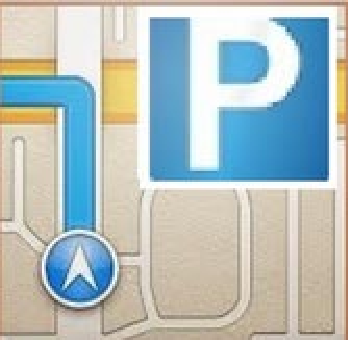
\includegraphics[scale=.6]{./analisisDeLaOferta/source/logo_aparcaCoches}
		\caption{Logo AparcaCoche}
		\label{fig:logo_aparcaCoches}
	\end{figure}

\paragraph{Descripci�n}
Aparcacoches es una aplicaci�n donde podr�s recordar autom�ticamente la posici�n del coche aparcado y llegar hasta �l sin ning�n tipo de problema. Adem�s podr�s anotar referencias adicionales para localizarlo y obtener informaci�n del punto donde te encuentras de forma instant�nea. B�sicamente con la aplicaci�n Aparcachoches podr�s:
\begin{itemize}
	\item Guardar la posici�n de tu coche aparcado
	\item Ver en el mapa tu posici�n actual y la del coche
	\item Trazar la ruta m�s cercana entre tu posici�n y la del coche
	\item Anotar referencias adicionales sobre el aparcamiento de tu coche: Parking, plaza de parking, etc
	\item Obtener direcci�n y coordenadas de tu posici�n actual, del coche y de cualquier punto del mundo
	\item Obtener distancias entre tu coche y tu posici�n actual
	\item Cambiar preferencias de visualizaci�n en el tipo de mapa, animaciones de posicionado, c�lculo de coordenadas, c�lculo de distancias, etc.
	\item Recibir ayuda sobre cualquiera de estas funciones anteriores a trav�s de unas instrucciones bien detalladas en la aplicaci�n
	\item �Ya no olvidar�s jam�s donde aparcaste tu coche!
\end{itemize}


\paragraph{Precio}
	Gratis

\paragraph{Plataformas}
	\begin{itemize}
		\item Android
	\end{itemize}
	
\paragraph{Link}
	\begin{itemize}
		\item \url{https://play.google.com/store/apps/details?id=com.lumibasqui.mapas}
	\end{itemize}
		
	\subsubsection{WIMC (�D�nde est� mi coche?)}
		\paragraph{Logo}
	Figura \ref{fig:logo_WIMC}
	\begin{figure}[h]
		\centering
		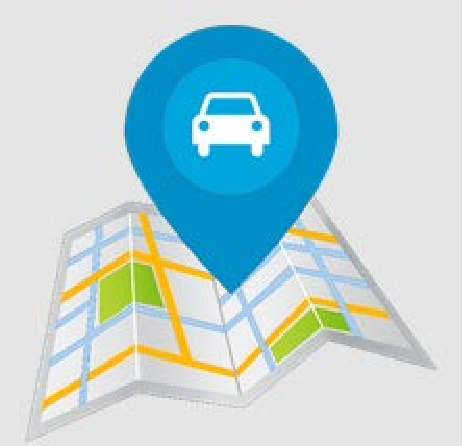
\includegraphics[scale=.6]{./analisisDeLaOferta/source/logo_WIMC}
		\caption{Logo WIMC}
		\label{fig:logo_WIMC}
	\end{figure}

\paragraph{Descripci�n}
Descripci�n
�Alguna vez estacionaste tu coche y se te olvid� d�nde lo hab�as dejado?
WIMC (Where's my car?) te permite guardar la posici�n de tu coche para que ya no lo vuelvas a perder.
Adem�s, permite obtener las indicaciones para llegar desde tu posici�n hasta el coche a trav�s de Google Maps y ver la informaci�n de los �ltimos lugares donde estacionaste.

Caracter�sticas:
\begin{itemize}
	\item Guardar la posici�n de tu coche.
	\item Obtener indicaciones sobre c�mo llegar.
	\item Informaci�n sobre �ltimos lugares, con fecha y tiempo de estacionamiento.
\end{itemize}

Pr�ximamente:
\begin{itemize}
	\item Guardar posici�n autom�ticamente cuando el dispositivo se desconecta del Bluetooth del coche.
	\item Sugerir posici�n autom�ticamente al detectar una pausa en el movimiento.
	\item Configuraciones de la aplicaci�n.
	\item Agregar comentario opcional al guardar la posici�n.
	\item Widget para guardar posici�n.
\end{itemize}

\paragraph{Precio}
	Gratis

\paragraph{Plataformas}
	\begin{itemize}
		\item Android
	\end{itemize}
	
\paragraph{Link}
	\begin{itemize}
		\item \url{https://play.google.com/store/apps/details?id=com.matiasguerra.wimc.app}
	\end{itemize}
		
	\subsubsection{Aparkando}
		\paragraph{Logo}
	Figura \ref{fig:logo_parkando}
	\begin{figure}[h]
		\centering
		
\includegraphics[scale=.6]{./analisisDeLaOferta/source/logo_parkando}
		\caption{Logo Parkando}
		\label{fig:logo_parkando}
	\end{figure}

\paragraph{Descripci�n}
Parkando es una nueva forma de conseguir estacionamiento en las diferentes ciudades del mundo. Si vas a un recital, cine o teatro, pod�s ahorrar tiempo y dinero encontrando el estacionamiento que m�s se ajuste a tus necesidades.
\\
Te permite:
\begin{itemize}
	\item Encontrar estacionamientos cercanos a donde est�s o ingresando una direcci�n
	\item Te permite ver los precios y horarios de los estacionamientos
	\item Pod�s ver c�mo llegar a un estacionamiento desde donde est�s
	\item Si conoc�s alg�n estacionamiento que no est� disponible en Parkando, lo pod�s crear.
	\item Se puede filtrar por distancia, precio, cochera fija, cochera m�vil y zona trapito.
\end{itemize}

\paragraph{Precio}
	Gratis

\paragraph{Plataformas}
	\begin{itemize}
		\item Android
	\end{itemize}
	
\paragraph{Link}
	\begin{itemize}
		\item \url{https://play.google.com/store/apps/details?id=ar.com.parkandoandroid&hl=es_419}
	\end{itemize}
		
	\subsubsection{Localizador de carro}
		\paragraph{Logo}
	Figura \ref{fig:logo_localizadorDeCarro}
	\begin{figure}[h]
		\centering
		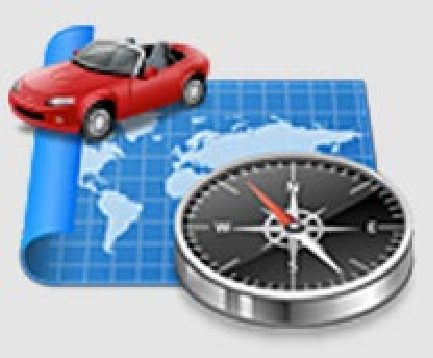
\includegraphics[scale=.6]{./analisisDeLaOferta/source/logo_localizadorDeCarro}
		\caption{Logo Localizador De Carro}
		\label{fig:logo_localizadorDeCarro}
	\end{figure}

\paragraph{Descripci�n}
Utilizar el buscador de coches a aparcar el coche y encontrar de nuevo m�s tarde. Esta aplicaci�n utiliza la configuraci�n de su tel�fono GPS para determinar donde est� su coche en relaci�n con usted. Los mapas se proporcionan para ayudarle a encontrar su coche. Park ilimitado coches, al mismo tiempo. Lleve un registro de tiempo en el parqu�metro. Puede introducir una descripci�n de su espacio de estacionamiento, y encontrar su coche utilizando el modo de br�jula o el modo de mapa. Coche Parker proporciona la distancia en kil�metros \/ metros o millas \/ yardas.
\\
\begin{itemize}
	\item Nunca pierda su coche aparcado de nuevo
	\item Parque ilimitada coches al mismo tiempo
	\item Lleve un registro de tiempo en el parqu�metro
	\item Utilice unidades m�tricas de Imperial
	\item Guardar la descripci�n de su lugar de estacionamiento
\end{itemize}

\paragraph{Precio}
	Gratis

\paragraph{Plataformas}
	\begin{itemize}
		\item Android
	\end{itemize}
	
\paragraph{Link}
	\begin{itemize}
		\item \url{https://play.google.com/store/apps/details?id=com.suderman.carparkerlite&hl=es}
	\end{itemize}
		
	\subsubsection{Parker}
		\paragraph{Logo}
	Figura \ref{fig:logo_Parker}
	\begin{figure}[h]
		\centering
		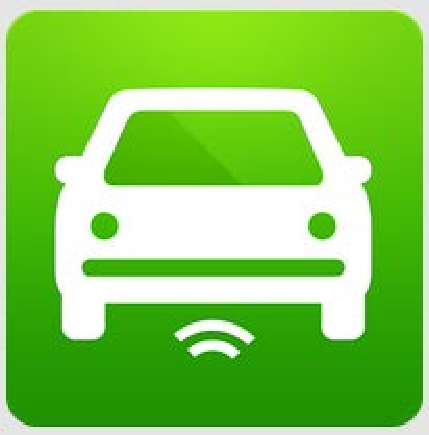
\includegraphics[scale=.6]{./analisisDeLaOferta/source/logo_Parker}
		\caption{Logo Parker}
		\label{fig:logo_Parker}
	\end{figure}

\paragraph{Descripci�n}
Parker shows you where open parking spaces are right now in more than 30 cities and universities in the US and the UK, while also giving you access to information for over 24,000 parking lots and garages. Simply select a street with available spots or garage on the map and get turn-by-turn voice navigation. You'll also get instant access to prices, payment options, and hours.
Up to the minute parking availability is offered in Los Angeles, Hollywood, Boston, Venice Beach, Studio City, Indianapolis, Reno, Fort Lauderdale and Ellicott City MD, as well as at Clemson University and Oregon State University, with more on the way. To see a longer list, scroll below.


Features of Parker include: 
\begin{itemize}
	\item Find open parking spots, and even see on which side of the street you'll find them 
	\item Use filters to only show spots that meet your preferences. (No coins? Not a problem ? we can show you where bills or credit cards are accepted; Need accessible parking? We can show you availability for that, too.) 
	\item View prices, payment options, hours (i.e., street parking free after 7PM), and more 
	\item One touch, turn-by-turn voice navigation quickly directs you to your preferred parking location 
	\item Built-in timer reminds you when your meter is about to expire 
	\item \textit{Walk-to-Car} provides directions back to your car 
	\item View traffic conditions en route to your destination
\end{itemize}

\paragraph{Precio}
	Gratis

\paragraph{Plataformas}
	\begin{itemize}
		\item Android
	\end{itemize}
	
\paragraph{Link}
	\begin{itemize}
		\item \url{https://play.google.com/store/apps/details?id=com.streetline.parker&hl=es}
	\end{itemize}
			
	\subsubsection{ParkMe Parking}
		\paragraph{Logo}
	Figura \ref{fig:logo_parkMe}
	\begin{figure}[h]
		\centering
		
\includegraphics[scale=.6]{./analisisDeLaOferta/source/logo_parkMe}
		\caption{Logo ParkMe}
		\label{fig:logo_parkMe}
	\end{figure}

\paragraph{Descripci�n}
Park your car smarter and faster with ParkMe, the world's largest and most accurate database of parking info.
Download our free award-winning parking app, now available on Android to find the cheapest, closest parking around! Check out our features:
\begin{itemize}
	\item View informative maps of parking lots and garages in your area.
	\item Check parking rates, see prices laid out on the map and compare costs
	\item Set our parking timer to help you avoid overstaying, overpaying or getting a ticket.
	\item See real-time info on exactly how many spots are open in a particular garage or lot. (Select markets only)
	\item When you decide on a lot or garage, get directions to the nearest driveway -- not just the street address.
\end{itemize}
 
Why circle the block wasting gas and time and fraying your nerves? Whether you're looking for city parking, sports parking or special event parking, Park Me has it covered. Get parking info before you leave the house, or pull over and use the app when you're close to your destination. With prices laid out on Park Me maps, you can always easily compare parking options.
The database at Park Me contains parking spots in over 500 cities around the world.
United States: 
\begin{itemize}
	\item Los Angeles
	\item San Francisco
	\item New York
	\item Seattle
	\item  Austin
	\item Houston
	\item Washington D.C.
	\item San Diego
	\item Santa Monica
	\item Denver
	\item Chicago
	\item Atlanta
	\item Philadelphia
	\item Dallas
	\item Boston
	\item Phoenix
	\item New Orleans
	\item Portland
	\item  Miami
	\item ...
\end{itemize}

Canada
\begin{itemize}
	\item Ottawa
	\item Vancouver
	\item Montrea
	\item Toronto
	\item Edmonto
	\item Calgary
	\item Winnipeg
	\item Quebec City
	\item ...
\end{itemize}

Europe
\begin{itemize}
	\item London
	\item Paris
	\item Madrid
	\item Rome
	\item Munich
	\item Frankfurt
	\item Prague
	\item Vienna
	\item ...
\end{itemize}
Plus hundreds of other cities.
Can't find parking in your city? Is a rate incorrect? Park Me wants to know! We add and update places to park every day. If you have any other suggestions or requests, we'd love to hear from you as well (@ParkMe).

\paragraph{Precio}
	Gratis

\paragraph{Plataformas}
	\begin{itemize}
		\item Android
	\end{itemize}
	
\paragraph{Link}
	\begin{itemize}
		\item \url{https://play.google.com/store/apps/details?id=com.parkme.consumer&hl=es}
	\end{itemize}
				
	\subsubsection{ParkMe Parking}
		\paragraph{Logo}
	Figura \ref{fig:logo_MeoParking}
	\begin{figure}[ht]
		\centering
		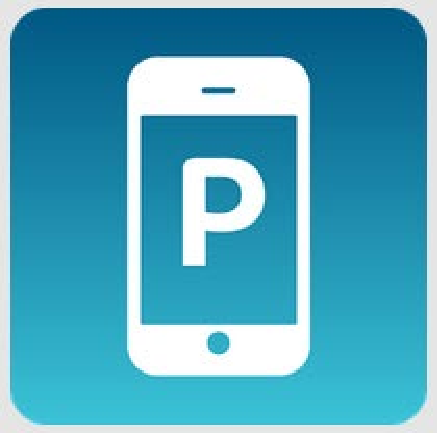
\includegraphics[scale=.6]{./analisisDeLaOferta/source/logo_MeoParking}
		\caption{Logo MEO Parking}
		\label{fig:logo_MeoParking}
	\end{figure}

\paragraph{Producto}
	MEO Parking


\paragraph{Descripci�n}
	
	�Pagar el aparcamiento con el tel�fono m�vil de una forma sencilla, segura y c�moda!
	El MEO Parking es un servicio que permite pagar el aparcamiento en la calle a trav�s del tel�fono m�vil, habiendo sido espec�ficamente dibujado para responder a las necesidades como pagar el aparcamiento sin hora de fin definida, pagar por valor o tiempo en diferentes zonas, entre otras especificidades.
	Proporciona una forma sencilla y alternativa, con autonom�a y comodidad a�adidas, de pagar el aparcamiento al permitir el pago en cualquier lugar y a cualquier hora.
	M�s alternativas de pago
	No necesita preocuparse con el hecho de no llevar suelto
	M�s autonom�a y comodidad
	No tiene que prever el tiempo que va a tardar
	Paga y prolonga el aparcamiento remotamente
	Mejor control del per�odo de aparcamiento
	Antes que el aparcamiento expire env�a un mensaje para el dispositivo m�vil a alert�ndole del acercamiento de su fin
	Disminuci�n de multas por transgresiones
	Paga el aparcamiento a mitad de una reuni�n, de una pel�cula o de un paseo
	Gesti�n On-line del servicio de aparcamiento
	Encuentra tu coche f�cilmente utilizando la funci�n de "encontrar un coche"
	

\paragraph{Precio}
	Gratis

\paragraph{Plataformas}
	\begin{itemize}
		\item Android
		\item iOS
	\end{itemize}
	
\paragraph{Link}
	\begin{itemize}
		\item \url{http://meoparking.pt/}
		\item \url{https://play.google.com/store/apps/details?id=ptsi.mobileparking.appandroid2.activities}
	\end{itemize}
				
	\subsubsection{Resumen}
		\input{./analisisDeLaOferta/resumenSolucionesUsuarioFinal}
	\chapter{Estudio de Viabilidad}
			\section{Definici�n Del Problema}
			En la actualidad se ha vuelto un problema cotidiano encontrar un lugar disponible en un estacionamiento, principalmente en zonas comerciales, de oficinas o de gran actividad econ�mica. Es com�n que un conductor (usuario) vaya a un estacionamiento en espec�fico y no encuentre un espacio disponible, lo cual puede hacer que pierda un tiempo considerable en encontrar un lugar disponible. 

Una investigaci�n realizada por el Instituto de Pol�ticas para el Transporte y el Desarrollo (ITDP), revel� que en �reas d�nde la oferta de estacionamientos no es suficiente para cubrir la demanda y se ofrecen espacios de estacionamiento en v�a p�blica de manera gratuita, se generan efectos negativos que afectan a residentes y visitantes \cite{ITDP}.

\begin{figure}[h]
	\centering
	\includegraphics[scale=.25]{./definicionDelProblema/source/trafico.pdf}
	\caption{Problemas cotidianos por falta disponibilidad en estacionamietos}
	\label{fig:ProblemasCotidianos}
\end{figure}

\begin{itemize}
	\item Baja disponibilidad de estacionamientos
	\item Estacionamientos ilegales
	\item Apropiaci�n ilegal de estacionamientos
	\item Altos niveles de ruido y contaminaci�n
	\item Congesti�n vial y tiempos de b�squeda largos en estacionamientos	
\end{itemize}


Por otro lado en estacionamientos(administradores) peque�os y medianos los ingresos no son suficientes para la adquisici�n de un sistema o la contrataci�n de  un  agente  externo  que  realice  dichas  administraci�n;  incluso  para  estacionamientos  grandes  con  mayores  ingresos  la implementaci�n de un sistema, automatizaci�n u outsourcing disminuye en gran medida sus ingresos.	
	\chapter{Especificaciones y requerimientos de software}
		\section{Requerimientos Funcionales}
\subsection{Administrador}

	\hrulefill
	\subsubsection{Visivilidad}
		Los administradores podr�n elegir si el estacionamiento es visible para todos los usuarios o solo para usuarios finales que autorice.
		
	\hrulefill	
	\subsubsection{Tipos de estacionamiento}
			\begin{itemize}
				\item \textbf{\textit{Estacionamiento c/s Pensi�n}} Ser�n estacionamientos donde los usuarios finales busquen un caj�n disponible donde aparcar su veh�culo. Al registar un nuevo estacionamiento de este tipo se podr� agrupar los cajones por \textbf{Nivel}(representan los pisos de los estacionamientos que cuenten con m�s de un nivel) y \textbf{Grupo} (agrupaci�n adicional que sive para ubicar en que bloque del estacaionamiento esta el caj�n). A cada caj�n se le podr� asignar un o varios pensionados, e indicar si estara reservado para discapacitados.
				
				\item \textit{Valet Parking} Es un servicio de aparkamiento que se le da a los usuarios. En este modelo los usuarios dejan su veh�culo en resepci�n y los encargados se ocupan de llevar el veh�culo hasta el estacionamiento. Para este tipo de estacionamientos el administrador podr� dar de alta uno o varios estacionamientos donde podran estacionar los veh�culos, cada estacionamiento del valet podra contara con Niveles, Gurpos y cajones.
				
				\item \textit{Parqu�metros} Son los estacionamientos que estan en calles p�blicas y pueden ser utilizados por cualqueira. Para este tipo de estacionamietos el administrador pued dar de alta zonas. Una zona representa una calle o calles donde se pueden haber N lugares para aparkar vehpiculos.
			\end{itemize}
			
	\hrulefill	
	\subsubsection{Pensionados con multiples veh�culos}
		El administrador podr� indicar si al reservar un caj�n a un pensionado este puede hacer uso de el solo con un veh�culo o con varios.
		
	\hrulefill	
	\subsubsection{Forma de estacionamiento}
		El administrador tendra la opcion de cargar una plantilla(croquis) del estacionamiento para representar la distribucion del estacionamiento.

	\hrulefill	
	\subsubsection{Consultas}
		Realizar� consultas de entradas-salidas e ingresos por:
		\begin{itemize}
			\item D�a
			\item Usuario
			\item Fecha
		\end{itemize}

	\hrulefill	
	\subsubsection{Entradas\/Salidas}
		Llevar� el control �ptimo de entradas y salidas de veh�culos.

	\hrulefill	
	\subsubsection{Modos de cobro}
		Manejara los siguientes modos de cobros:
		\begin{itemize}
			\item Por hora
			\item Por minuto
			\item Por Estancia
			\item Primeros n minutos, con incremento cada n minutos
			\item Boleto perdido
			\item Boleto no sellado
			\item Sin cobro
		\end{itemize}

	\hrulefill	
	\subsubsection{Tarifas especiales}
		El sistema permitir� agregar precios especiales como promociones para clientes.

	\hrulefill	
	\subsubsection{Historial}
		Llevar� un historial donde se registrar�n los movimientos realizados en el estacionamiento, estos detallaran los cajones, hora de entrada, hora de salida y la cantidad cobrada.
	
	\hrulefill	
	\subsubsection{Habilitar reservaci�n}
		Podr� habilitar o desbilitar la opci�n de \textit{Reservacion de Caj�n} para su estacionameinto. En caso de hanilitarlo deber� indicar la tolerancia para que el usuario acceda al estacionamiento, en caso contrario perdera su reservaci�n.

	\hrulefill	
	\subsubsection{Control de usuarios}
		Ppodr� gestionar las cuenta de los operadores.
	
	
\subsection{Usuario Final}

	\hrulefill	
	\subsubsection{Reservaciones}
		Podr� hacer una reservaci�n de un caj�n de estacionamiento previamente seleccionado desde la aplicaci�n m�vil.
	\hrulefill	
	\subsubsection{Historial de usuario}
		Podr� llevar un control sobre los estacionamientos visitados, as� como aquellos seleccionados por este como favoritos.
	\hrulefill	
	\subsubsection{Busqueda de estacionamientos}
		Podr� seleccionar un radio m�ximo de metros a la redonda en donde ser�n visualizados los estacionamientos.
	\hrulefill	
	\subsubsection{Visualizacion de smartphone}
		Podra� visualizar en un dispositivo movil(smarphone) los estacionamientos cercanos a su ubicacion dados de alta en el sistema, mostrando informaci�n del estacionamiento al seleccionarlo. 
		\begin{itemize}
			\item Horario de operac�n
			\item Capacidad y cajones disponibles.
			\item Modos de cobro
			\item Servicios adicionales
			\item Tarifas especiales
		\end{itemize}
\section{Requerimientos No Funcionales}
\hrulefill
	\subsubsection{SaaS}
	El sistema trabajar� bajo una plataforma Cloud, y sera accedido como un servicio.

\hrulefill
\subsubsection{Seguridad}
	Toda la informaci�n deber� ser accedida y manipulada solo por el personal autorizado.

\hrulefill
\subsubsection{Comparar estacionamientos}
	Al buscar los estacionamientos cercanos desde la App se deber� indicador de manera visual la calificacion de cada estacionamiento obtenida con los datos del sistema.
\section{Reglas de negocio}
\subsection{RNF}
	\paragraph{Alta de stacionamiento}
		Los datos para dar de alta un estacionamiento son:
		\begin{itemize}
			\item Nombre del estacionamiento.
			\item Ubicaci�n(texto y coordenadas geogr�ficas)
			\item Logo representativo (Opcional)
			\item Horario de servicio  
			\item N�mero de niveles y cajones por nivel
			\item Cajones para personas con capacidades diferentes
		\end{itemize}

\subsection{RNF}
	\paragraph{Reservaci�n}
		Para que el usuario final pueda reservar un caj�n, tendra que ingresar el n�mero de placa del veh�culo.   

\subsection{RNF}
	\paragraph{SaaS}
		El sistema trabajar� bajo una plataforma Cloud, y ser� accedido como un servicio API.

\subsection{RNF}
	\paragraph{Configuraci�n de estacionamiento}
		Un estacionameito podr� operar con las siguientes configuraciones.
		\begin{itemize}
			\item Estacionamiento 
			\item Pensi�n
			\item Valet
			\item Estacionamiento con Pensi�n 					
		\end{itemize}

\subsection{RNF}
	\paragraph{N�mero de accesos}
		Los estacionamientos tpodr�n tener de uno a muchos accesos. Estos acceos es donde se registrarn entradas y salidas.

\subsection{RNF}
	\paragraph{Horario de pensi�n}
		Al registrar un pensionado se deber� indicar.
		\begin{itemize}
			\item Placas del veh�culo 
			\item Horario de uso
			\item Vegencia de uso			
		\end{itemize}
		
\subsection{RNF}
	\paragraph{Tiempo de vida de la informaci�n}
		La informaci�n ser� alamcenada en el sistema, pero no se�a eliminada.
		
		
\section{Stakeholders}
\hrulefill
\subsubsection{CAJERO}
	\paragraph{Descripci�n}
		Persona que operar� el sistema desde una cabina.
	\paragraph{Responsabilidades}
		Registrar las entradas y salidas, ademas realizar los cobros a los usuarios finales.
	\paragraph{Ubicaci�n}
		Acesso del estacionamiento
	\paragraph{Cantidad}
		Depende el n�mero de accesos que se tenga en el estacionamiento

\hrulefill
\subsubsection{ADMINISTRADOR}
	\paragraph{Descripci�n}
		Persona se encarga del la administraci�n del estacionameinto
	\paragraph{Responsabilidades}
		Configuraci�n del sistema. Gresti�n de cuanetas de usuario. 
	\paragraph{Cantidad}
		1

\hrulefill
\subsubsection{USUARIO FINAL}
	\paragraph{Descripci�n}
		Persona que accesa desde la aplicaci�n mov�l.
	\paragraph{Responsabilidades}
		\begin{itemize}
			\item Reservaaci�n
			\item Calificar estacionamientos
		\end{itemize}
	\paragraph{Cantidad}
		n
	
			
			
\end{document}